\chapter{State of the Art}\label{sec:state-of-the-art}

In this chapter, the current situation and state-of-the-art models are
discussed. In Section \ref{sec:scope}, the scope of the thesis is defined and
the methodology of selecting related work is described. After this related
work on the topics of \gls{rl}-based schedulers, assessing the robustness of
\gls{rl} methods and approaches for reducing retraining time are discussed.
Lastly, the gap in the related work is analysed.


\section{Scope and Methodology}\label{sec:scope}

The scope of this thesis is specifically \gls{rl}-based schedulers in cloud
environments. In Section \ref{sec:rl}, it is explained why this thesis only
focuses on \gls{rl}-based schedulers, not schedulers based on other forms of
\gls{ml}.

Comparing different methods and models is the main task in this thesis. When
comparing methods of models, a justified method of assessing methods and models
is required. It is also important that the comparison is made on the
indicators on which the performance depends. These are called the \glspl{kpi}. The
\glspl{kpi} of \gls{rl}-based schedulers are established from related literature.

The methodology of the research in related work is twofold. Most of the work
of others is discovered via Google Scholar\footlink{scholar.google.com}. This
search engine searches through known scientific databases, e.g.
arXiv\footlink{arxiv.org}, Research Gate\footlink{researchgate.net}, and
additionally universities' websites, e.g. from the University of
Amsterdam\footlink{uva.nl}. The other method for finding related work is by
reading literature referenced in earlier found related work.


\section{Related Work}

\subsection{Reinforcement-Learning-based Schedulers}\label{sec:rl}

Reinforcement learning, as it does not rely on labeled data and its
interactive learning process, gets widely used in scheduling. This difference
is very well explained in `the most popular artificial intelligence textbook
in the world'\footnotemark, \citeA{russell2010}. Their explanation of \gls{rl} is
summarised in the following paragraph.

\footnotetext{According to \href{\urltor}{this blog}, but also shown on the
homepage of the book (\url{http://aima.cs.berkeley.edu/}).}

Reinforcement learning is one of the three basic paradigms in machine
learning, along with supervised learning and unsupervised learning. \gls{rl} is
different from the other two paradigms. Supervised learning and unsupervised
learning have a shared property: the need for data. Supervised learning needs
annotated data, various inputs and desired outputs are given, and the
algorithm learns a function to get as close to the wanted outputs as possible
given the inputs. With unsupervised learning, a model is forced to build an
internal representation of the world by mimicking the data. \gls{rl} is different
because it does not depend on data, but rather learns from a feedback loop of
rewards or reinforcements. It typically consists of one agent, a set of
actions and a set of states. The agent accumulate rewards by performing series
of actions in the environment. See Figure \ref{rl-diagram} for a flowchart of
reinforcement learning. In many complex environments \gls{rl} can be the most
feasible method for training models because there might be little data
available or the environment is too complex to model \cite{russell2010}. For
the reason that \gls{rl} does not need large amounts of data but an environment to
interact via actions and rewards, lots of work has been done with
investigating \gls{rl}-based scheduling approaches.

\begin{figure}[htp!]
    \centering
    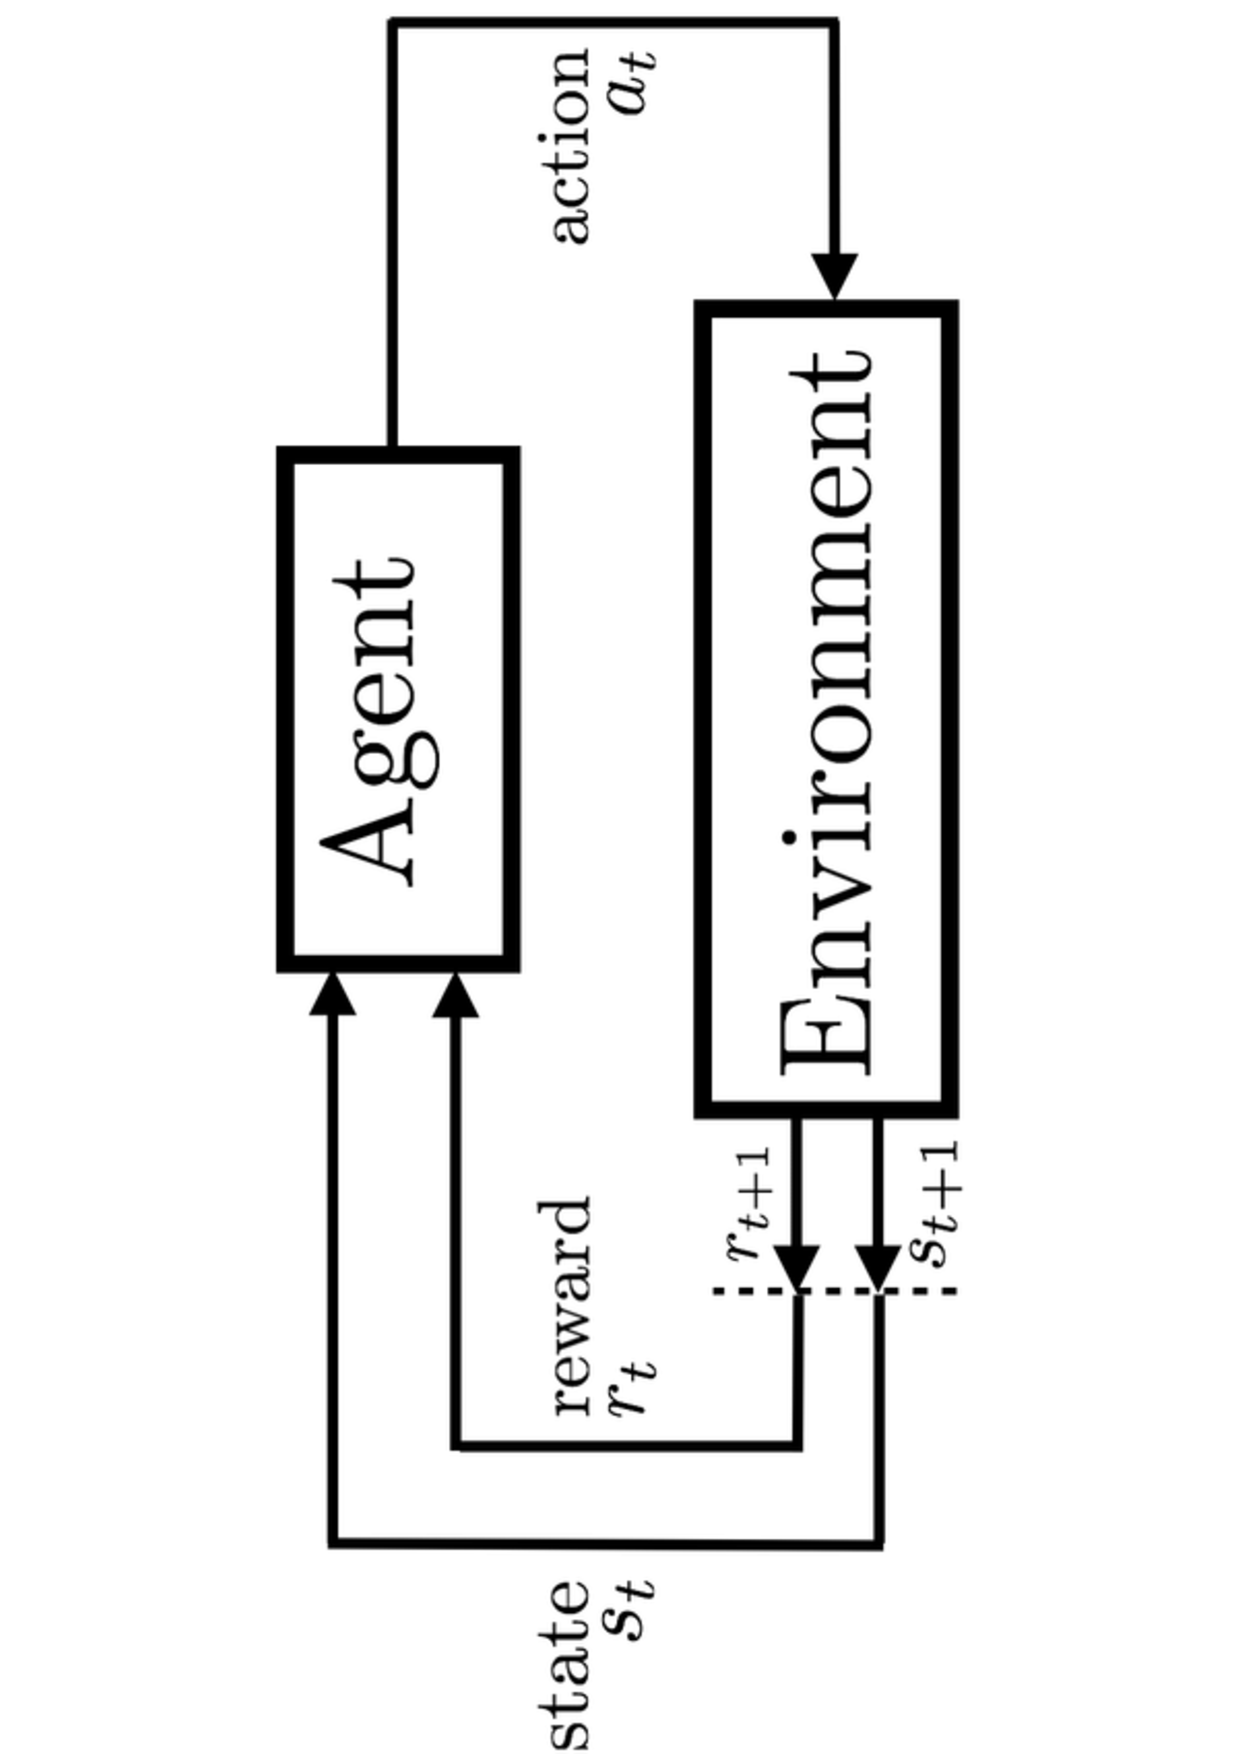
\includegraphics[angle=-90,width=.5\textwidth]{./fig/rl-diagram.pdf}
    \caption{During a trial $t$ the agent receives the state $s_t$ and
    performs an action $a_t$ in this state. After the action, it receives
    the new state $s_{t+1}$ and a reward for the action $r_{t+1}$ from the
    environment \protect\cite{rafati2019}.}
    \label{rl-diagram}
\end{figure}


Many reinforcement learning algorithms are used in state-of-the-art
\gls{rl}-based schedulers. Three different state-of-the-art \gls{rl}
schedulers are described. The first scheduler is DeepRM, presented in
\citeA{mao2016}. This scheduler is based on deep reinforcement learning with
policy representation via a \gls{dnn}. The algorithm learns by performing
gradient-descent on the policy parameters using the REINFORCE algorithm from
\citeA{sutton1999}. For the state representation, a 2-D image is used to
capture the status of resources and jobs. The second state-of-the-art
scheduler is proposed in \citeA{zhang2020} and also trains a policy network,
but in this algorithm, the network is trained using \ppo, an actor-critic
algorithm. Unlike DeepRM, the model from \citeA{zhang2020} is not hard bounded
by the instance size \cite[p.~5]{zhang2020}, making it more flexible and
robust. Lastly, \citeA{wang2020} is a state-of-the-art scheduler, but since it
uses meta-learning it is discussed in Section \ref{sec:reusing}. In Table
\ref{rlschedulers}, some results of the related work discussed in this
paragraph are listed. The results show that all \gls{rl}-based schedulers are
an improvement on schedulers based on heuristics.

\begin{table}[htp!]
    \centering
    \caption{Achievements from \gls{rl}-based job schedulers as shown in their
    paper. The achievements are compared in their papers to heuristic-based
    approaches.}
    \label{rlschedulers}
    \resizebox{\textwidth}{!}{
    \begin{tabular}{p{4.2cm}||l|l|l}
        Literature & \protect\citeA{mao2019} & \protect\citeA{wang2020} & \protect\citeA{zhang2020}\\ \hline
        Name & Decima & MRLCO & -\\
        Metric & \jct & Latency & Objective\footnotemark\\
        Baseline & \gls{fifo} & Greedy Heuristic & \sjf\\
        Performance Deviation (result / baseline) & 61.1s / 111.4s & 743.42ms / 893.62ms &
        2508.28 / 3208.69\\
    \end{tabular}
    }
\end{table}

\footnotetext{Average of the makespan, flowtime and tardiness.}



\subsection{Evaluation of Reinforcement Learning Models}\label{sec:evaluation}

Finding approaches to effectively assess and compare \gls{rl}-based schedulers is a
sub-question of this thesis and, by that, a key factor to answer the research
question. \gls{rl}-based schedulers must be as effective after reducing retraining
time as before the reduction. In the reviewed related work, there was no
standard found for evaluating \gls{rl} models. Work is done in defining standard
evaluation methods, but these methods are not yet the industry standard. There
are three representative metrics adopted by many works. The first evaluation
is regret. Regret can only be used as a metric when an agent with optimal
policy can be defined. The difference in received reward for the actions taken
by the optimal agent and the learning agent is the regret per action. However,
knowing the optimal policy is not always possible. The second evaluation
metric is not used much among literature but rather in practice, namely the
OpenAI Gym. Gym provides well-defined environments that are suitable for
\gls{rl}
to learn. A comparison between \gls{rl} models is done on their
leaderboards\footlink{github.com/openai/gym/wiki/Leaderboard}. The metrics are
the number of episodes before `solve'. Some environments define being solved
as receiving an average reward threshold over 100 consecutive trials (when a
model is converged), and other environments have a clear goal which can be
achieved. Lastly, proposed methods in literature are, for example, a framework
for evaluating \gls{rl} in \citeA{khetarpal2018} and a novel evaluation method in
\citeA{jordan2020}. Both of these are not used often in practice. It can be
concluded that even though no standard exists, many approaches for evaluating
\gls{rl} models exist and are used.


\subsection{Assessing Robustness of Reinforcement Learning}

To select a method for reducing retraining time, it is vital to assess the
robustness of a model. Robustness is the ability to cope with dynamic
environments and working well in noisy environments. The goal of this thesis is
to compare methods for reducing the retraining time of \gls{rl}-based schedulers. If
a model is robust, it needs less time of adapting models to the new
environment, which results in less retraining time. Because less
retraining time can be achieved with more robustness, related work on robust
reinforcement learning algorithms is discussed. The comparison between
robustness of reinforcement learning models is only as descriptive as the
metric used for it. Selecting a well-formed method for assessing robustness is
essential for this research.

Many methods for assessing the robustness of reinforcement learning use some
``disturbance'' in the training environment \cite{morimoto2005}. By
changing dynamic aspects of the environment, the model learns about the
dynamics and accounts for this. Both of these methods require knowledge of the
dynamics in the environment and the ability to simulate the dynamics.

In \citeA{alnima2021} the neuron coverage, i.e. the ratio of the activated
neurons in a network, is used as a measurement of robustness. This is only
applicable in \gls{rl} methods with neural networks in it, for example
\gls{dqn}.

Another approach to evaluating robustness is training on data and
testing on completely other data. By evaluating the difference, the resulting
model can be compared on how well it performs on the same values versus how it
performs on other values. This is done in \citeA{pinto2017}, and other papers.


\subsection{Approaches to Reduce Retraining Time}\label{sec:reduce}

To answer the third sub-question, the current state-of-the-art approaches are
discussed. The approaches are categorised into three categories: (1) approaches
modelling the dynamic aspect of the environment, (2) approaches using
adversarial agents and (3) approaches that reduce retraining by using earlier
learned policies. The reviewed approaches to reduce retraining time are
discussed on categorical basis in the following sections.


\subsubsection{Modelling the Dynamic Environment}\label{sec:model}

Modelling the dynamics of the environment is a straightforward approach to
taking the dynamics into account. For example, for job schedulers in cloud
environments, this can be done by dynamically adding and removing resources
during training. It theoretically helps the agent to learn the knowledge of
dynamics. Numerous approaches include information about the dynamic aspect of
the environment in the model. To successfully apply \gls{rl} models in dynamic
environments, \citeA{wiering2001} proposed to include an a priori model of the
changing parts in the environment. In \citeA{nagayoshi2013}, a method was
proposed for detecting environmental changes on which the model can adapt. The
aforementioned proposed methods require a model of the environment or a priori
knowledge of the changing parts of the environment. In many environments, this
would not be feasible, but it could be possible in job scheduling since there
are not many dynamics that can change. The disadvantage of modelling the
dynamic environment is that lots of data is needed for modelling dynamics.
Another approach to modelling dynamics is letting the dynamics randomly
happen. It is unsure if this would actually work. Resource failure can be
predicted using state information about resource state. This is out of the
scope of this thesis.


\subsubsection{Adversarial Agents}\label{sec:adversarial}

Another approach for learning how to handle disturbance is by adding in a
disturbing agent \cite{morimoto2005}. The disturbing agent learns to perform
the most disturbing action as possible. The same approach is also proposed in
\citeA{pinto2017}, therein called robust adversarial reinforcement learning.
In \citeA{pinto2017}, it is also stated that the gap between simulation and
real world is too large for policy-learning approaches to work well. Good
working policy-learning approaches is achievable only if the adversarial agent
can control the time when specific resources are inserted or deleted. This raises
a number of questions. How would the number of operations (insertion and
deletions of resources) be selected? This has to be controlled otherwise the
adversarial agent would score best by deleting all resources. Will the agent
work better than training with random resource operations? Are there critical
moments where the deletion of resources is worse than other moments?

Implementing an adversarial agent can be performed with Q-learning models. \Ql is a
model typically used in single-agent environments and is simple. Having two
Q-learning agents in an environment, one learning the main task, and the other
being the adversarial agent, can improve robustness. This technique has been
used in a simple two-player game \cite{littman1994}. There are also other
approaches for reducing retraining time of \ql models in specific. These
approaches include `repeated update Q-learning' \cite{abdallah2016} and variants
of \dqn like robust \dqn \cite{chen2018}.

Another approach is to train robustly online, i.e. during deployment of the
model \cite{fisher2019}. This approach, called Robust Student-\dqn (RS-\dqn)
deploys adversarial agents online to trick the model into unwanted states.
This approach maintains competitive performance.


\subsubsection{Meta-Learning}\label{sec:reusing}

Meta reinforcement learning is a method for learning to quickly adapt online
to new tasks. Adapting is done in the context of model-based reinforcement
learning. Meta reinforcement learning models use meta-learning to train a
dynamics model that can be rapidly adapted to local context
\cite{nagabandi2019}. Meta-learning is described as ``Learning to learn''. A
model is trained to learn during meta-training. Here, the learner learns the new
task and the meta-learner trains the learner. In \cite{schweighofer2003} it is
proposed to learn meta-parameters with stochastic gradients. It is a robust
algorithm that finds appropriate meta-parameters and controls the parameters
in a dynamic, adaptive manner. Even when retraining is needed to adapt to the
changes in the environment, the models parameters will probably be nearly the
same as before. Another meta-learner is the \mrlco model from
\citeA{wang2020}. In the article, a task offloading method based on meta
reinforcement learning is proposed. This model uses a sequence-to-sequence
neural network that is trained by order approximation and clipped surrogate
objectives. The model reduces latency by up to 25\% and can adapt fast
to new environments. After the first time learning, it requires much less
iterations to receive the same reward as previous training sessions.


\section{Gap Analysis}\label{sec:gap}

As shown in this chapter, much work is done in optimising job scheduling with
reinforcement learning. The popularity and convenience of \gls{rl} is the
reason it gets attention in the field of scheduling. Although much work is
done, there are still gaps in previous research. The reason to investigate
reducing retraining time is because conventional \gls{rl} is not robust enough
to deal with dynamic scheduling scenarios. Many state-of-the-art schedulers
using \gls{rl} outperform heuristic-based methods with great distance. The
downside of the \gls{rl}-based schedulers is that they lack the ability to
cope with the dynamics in the environment. Once dynamics occur in the
environment, the \gls{rl} model has to be retrained, which is time consuming.
Most of them are trained for a specific instance and did not train for
dynamics. Including these aspects in training, along with methods for reducing
retraining time or adding in robustness, can help reduce retraining time.
Although there exist methods for reducing the retraining time, these methods
have not been compared in \jss environments, trained on the same data. A
comparison is needed to help with selecting a well-suited method. \glspl{kpi}
have to be found on which these reduce methods can be selected. A standard for
assessing the robustness of models has not been found, but combining multiple
can have the desired result. To summarise, the gaps in previous done research are the
following:
\begin{itemize}[noitemsep]
    \item Conventional \gls{rl} is not robust enough to deal with dynamic
        scheduling scenarios;
    \item \gls{rl}-based schedulers lacking robustness require more retraining time,
        which takes time, costs resources itself, costs money and contributes
        to global warming;
    \item There are no standards for assessing robustness of a model, but
        approaches from related literature can also be used here to assess
        the robustness;
    \item There has not been a comparative study of methods for adding in
        robustness of reducing retraining time in the same conditions.
\end{itemize}
This thesis will fill in the gap by providing a standardised method for
selecting approach to reduce retraining time. This is done by having a solid
approach for assessing robustness and overall performance of \gls{rl}-based
schedulers. The following chapter explains the methodology of filling in the
gaps.
